\chapter{Statistical Decision Theory}

\begin{ex}
  \begin{enumerate}[(a)]
    \item Let $X\sim\text{Binomial}(n,p)$ and take the prior
          $p\sim\text{Beta}(\alpha,\beta)$.
          \begin{align*}
            f(x\,|\,p)f(p)
             & \propto
            p^x(1-p)^{n-x}p^{\alpha-1}(1-p)^{\beta-1} \\
             & =p^{x+\alpha-1}(1-p)^{n+\beta-x-1},
          \end{align*}
          which normalizes to the PDF of a $\text{Beta}(\alpha+x,\beta+n-x)$
          distribution.

          By Theorem 12.8, the Bayes estimator is the mean of the posterior, and
          therefore
          \[
            \phat=\frac{\alpha+X}{\alpha+\beta+n}.
          \]

          Recall that
          \begin{align*}
            R(p,\phat)
             & =\mathbb{V}_p\left(\frac{\alpha+X}{\alpha+\beta+n}\right)
            +\left[\textsf{bias}_p\left(\frac{\alpha+X}{\alpha+\beta+n}\right)\right]^2       \\
             & =\frac{\mathbb{V}_p(X)}{(\alpha+\beta+n)^2}
            +\left[\frac{\alpha+np}{\alpha+\beta+n}-p\right]^2                                \\
             & =\frac{\mathbb{V}_p(X)}{(\alpha+\beta+n)^2}
            +\left[\frac{\alpha+np}{\alpha+\beta+n}-p\right]^2                                \\
             & =\frac{np(1-p)}{(\alpha+\beta+n)^2}
            +\left[\frac{\alpha-\alpha p-\beta p}{\alpha+\beta+n}\right]^2                    \\
             & =\frac{np(1-p)+(\beta p - \alpha(1-p))^2}{(\alpha+\beta+n)^2}                  \\
             & =\frac{\beta^2p^2+(n-2\alpha\beta)p(1-p)+\alpha^2(1-p)^2}{(\alpha+\beta+n)^2},
          \end{align*}
          and that therefore the Bayes risk is
          \begin{align*}
            r(f,\phat)
             & =\int_0^1\!R(p,\phat)f(p)\,\d{p}                                                    \\
             & =\frac{\beta^2B(\alpha+2,\beta)
              +(n-2\alpha\beta)B(\alpha+1,\beta+1)
              +\alpha^2B(\alpha,\beta+2)}{(\alpha+\beta+n)^2B(\alpha, \beta)}                      \\
             & =\frac{\beta^2\alpha(\alpha+1)+(n-2\alpha\beta)\alpha\beta+\alpha^2\beta(\beta+1)}{
              (\alpha+\beta+n)^2(\alpha+\beta)(\alpha+\beta+1)}                                    \\
             & =\frac{\alpha\beta}{
              (\alpha+\beta+n)(\alpha+\beta)(\alpha+\beta+1)},                                     \\
          \end{align*}
          since
          \begin{align*}
             & \int_0^1\!
            \beta^2p^{\alpha+2-1}(1-p)^{\beta-1}
            +(n-2\alpha\beta)p^{\alpha+1-1}(1-p)^{\beta+1-1}
            +\alpha^2p^{\alpha-1}(1-p)^{\beta+2-1}\,\d{p} \\
             & \quad=\beta^2B(\alpha+2,\beta)
            +(n-2\alpha\beta)B(\alpha+1,\beta+1)
            +\alpha^2B(\alpha,\beta+2).
          \end{align*}
    \item Let $X\sim\text{Poisson}(\lambda)$ and take the prior
          $\lambda\sim\text{Gamma}(\alpha,\beta)$. By Exercise 11.6, the
          posterior distribution of $\lambda$ is a
          $\text{Gamma}(\alpha',\beta')$ distribution with
          \[
            \alpha'=\alpha+x,\text{ and }
            \beta'=\frac{\beta}{\beta +1},
          \]
          and posterior mean (and therefore Bayes estimator),
          \[
            \widehat{\lambda}=\left(\alpha+x\right)
            \left(\frac{\beta}{\beta +1}\right).
          \]
          We have
          \[
            \mathbb{V}_\lambda\left(
            \widehat{\lambda}
            \right)
            =\mathbb{V}_\lambda\left(
            \left(\alpha+X\right)
            \left(\frac{\beta}{\beta +1}\right)
            \right)
            =\frac{\lambda\beta^2}{(\beta+1)^2},
          \]
          and
          \[
            \mathbb{E}_\lambda\left(
            \widehat{\lambda}
            \right)
            =\frac{(\alpha+\lambda)\beta}{\beta+1},
          \]
          and therefore
          \begin{align*}
            R(\lambda,\widehat{\lambda})
             & =\mathbb{V}_\lambda(\widehat{\lambda})
            +\left(\textsf{bias}_\lambda(\widehat{\lambda})\right)^2                       \\
             & =\frac{\lambda\beta^2}{(\beta+1)^2}
            +\left(\frac{\alpha\beta-\lambda}{\beta+1}\right)^2                            \\
             & =\frac{\lambda^2+\lambda\beta(\beta-2\alpha)+\alpha^2\beta^2}{(\beta+1)^2}.
          \end{align*}

          Since
          \begin{align*}
            \int_0^\infty\!
            \frac{1}{\beta^\alpha\Gamma(\alpha)}\lambda^{\alpha+2-1}e^{-\lambda/\beta}\,\d{\lambda}
             & =\alpha(\alpha+1)\beta^2\int_0^\infty\!
            \frac{1}{\beta^{\alpha+2}\Gamma(\alpha+2)}\lambda^{\alpha+2-1}e^{-\lambda/\beta}\,\d{\lambda}
            =\alpha(\alpha+1)\beta^2,                  \\
            \int_0^\infty\!
            \frac{1}{\beta^\alpha\Gamma(\alpha)}\lambda^{\alpha+1-1}e^{-\lambda/\beta}\,\d{\lambda}
             & =\alpha\beta\int_0^\infty\!
            \frac{1}{\beta^{\alpha+1}\Gamma(\alpha+1)}\lambda^{\alpha+2-1}e^{-\lambda/\beta}\,\d{\lambda}
            =\alpha\beta,
          \end{align*}
          it follows that
          \begin{align*}
            r(f,\widehat{\lambda})
             & =\int_0^\infty\!R(\lambda,\widehat{\lambda})f(\lambda)\,\d{\lambda}                         \\
             & =\frac{\alpha(\alpha+1)\beta^2+\alpha\beta^2(\beta-2\alpha)+\alpha^2\beta^2}{(\beta+1)^2}   \\
             & =\frac{\alpha\beta^2}{\beta+1}                                                            .
          \end{align*}
    \item Let $X\sim N(\theta,\sigma^2)$, with $\sigma^2$ known and the prior
          $\theta\sim N(a,b^2)$. By Exercise 11.1, we have
          \[
            \theta\,|\,X\sim N\left(\frac{b^2X+\sigma^2a}{\sigma^2+b^2},
            \frac{\sigma^2b^2}{\sigma^2+b^2} \right),
          \]
          and therefore the Bayes estimator is
          \[
            \thetahat=\frac{b^2X+\sigma^2a}{\sigma^2+b^2}.
          \]

          We have
          \[
            \mathbb{V}_\theta(\thetahat)
            =\mathbb{V}_\theta\left(\frac{b^2X+\sigma^2a}{\sigma^2+b^2}\right)
            =\left(\frac{\sigma b^2}{\sigma^2+b^2}\right)^2,\text{ and}
          \]
          \[
            \mathbb{E}_\theta(\thetahat)
            =\mathbb{E}_\theta\left(\frac{b^2X+\sigma^2a}{\sigma^2+b^2}\right)
            =\frac{b^2\theta+\sigma^2a}{\sigma^2+b^2},
          \]
          and therefore
          \begin{align*}
            R(\theta,\thetahat)
             & =\mathbb{V}_\theta(\thetahat)
            +\left(\textsf{bias}_\theta(\thetahat)\right)^2                                         \\
             & =\frac{\sigma^2b^4+\sigma^4a^2-2\sigma^4a\theta+\sigma^4\theta^2}{(\sigma^2+b^2)^2}.
          \end{align*}

          Since
          \[
            \int_{-\infty}^\infty\!
            \frac{\theta}{\sqrt{2\pi b^2}}
            \exp\left\{-\frac{(\theta-a)^2}{2b^2}\right\}\,\d{\theta}
            =0,\text{ and }
          \]
          \begin{align*}
             & \int_{-\infty}^\infty\!
            \frac{\theta^2}{\sqrt{2\pi b^2}}
            \exp\left\{-\frac{(\theta-a)^2}{2b^2}\right\}\,\d{\theta} \\
             & \quad = \int_{-\infty}^\infty\!
            \frac{(\theta+a)^2}{\sqrt{2\pi b^2}}
            \exp\left\{-\frac{\theta^2}{2b^2}\right\}\,\d{\theta}     \\
             & \quad =b\int_{-\infty}^\infty\!
            \frac{(bu+a)^2}{\sqrt{2\pi b^2}}
            \exp\left\{-\frac{u^2b^2}{2b^2}\right\}\,\d{u}            \\
             & \quad =b^2\int_{-\infty}^\infty\!
            \frac{(u+a/b)^2}{\sqrt{2\pi}}
            \exp\left\{-\frac{u^2}{2}\right\}\,\d{u}                  \\
             & \quad =b^2\int_{-\infty}^\infty\!
            \frac{u^2}{\sqrt{2\pi}}
            \exp\left\{-\frac{u^2}{2}\right\}\,\d{u}
            +a^2\int_{-\infty}^\infty\!
            \frac{1}{\sqrt{2\pi}}
            \exp\left\{-\frac{u^2}{2}\right\}\,\d{u}                  \\
             & \quad=a^2+b^2,
          \end{align*}
          it follows that
          \[
            r(f,\thetahat)
            =\int_{-\infty}^\infty\!R(\theta,\thetahat)f(\theta)\,\d{\theta}
            =\frac{\sigma^2(b^4+2\sigma^2a^2+\sigma^2b^2)}{(\sigma^2+b^2)^2}.
          \]
  \end{enumerate}
\end{ex}

\begin{ex}
  Recall that the risk of an estimator $\thetahat$ with respect to a loss
  function $L(\theta,\thetahat)$ is given by
  \[
    R(\theta,\thetahat)=\mathbb{E}_\theta(L(\theta,\thetahat))
  \]
  and that therefore if $L(\theta,\thetahat)=(\theta-\thetahat)^2/\sigma^2$
  and $L_\text{SL}$ is the ordinary square loss we have
  \[
    R(\theta,\thetahat)=\mathbb{E}_\theta(L(\theta,\thetahat))
    =\mathbb{E}_\theta\left(\frac{1}{\sigma^2}L_\text{SL}(\theta,\thetahat)\right)
    =\frac{1}{\sigma^2}\mathbb{E}_\theta\left(L_\text{SL}(\theta,\thetahat)\right),
  \]
  which is a constant multiple of the squared error risk. Hence, since $\Xbar$
  is admissible under the squared error loss by Theorem 12.20, it is also
  admissible under the loss $L$.

  We have
  \begin{align*}
    \mathbb{E}_{\theta}\left(\frac{(\theta-\Xbar)^2}{\sigma^2}\right)
     & =\frac{\theta^2-2\theta\mathbb{E}_\theta(\Xbar)+\mathbb{E}_\theta(\Xbar^2)}{\sigma^2}    \\
     & =\frac{\theta^2-2\theta^2+\mathbb{V}_\theta(\Xbar)+\mathbb{E}_\theta(\Xbar)^2}{\sigma^2} \\
     & =\frac{\theta^2-2\theta^2+\sigma^2/n+\theta^2}{\sigma^2}                                 \\
     & =\frac{1}{n},
  \end{align*}
  and therefore, by Theorem 12.21, since $\Xbar$ has constant risk and is
  admissible, it follows that it is also minimax.
\end{ex}

\begin{ex}
  Recall that the Bayes estimator is the one that minimizes the posterior risk
  $r(\thetahat\,|\, x)$. We have
  \begin{align*}
    r(\thetahat\,|\, x)
     & =\sum_{i=1}^k L(\theta_k,\thetahat)f(\theta_k\,|\,x)           \\
     & =\sum_{i=1}^k I_{\{\theta_k\}^c}(\thetahat)f(\theta_k\,|\,x)   \\
     & =\sum_{i=1}^k (1-I_{\{\theta_k\}}(\thetahat))f(\theta_k\,|\,x) \\
     & =k-f(\thetahat\,|\,x),
  \end{align*}
  which is minimized by the choice of $\thetahat$ that maximizes the posterior
  likelihood. But this is precisely the posterior mode.
\end{ex}

\begin{ex}
  Let $\sigmahat^2=bS^2$ where $S^2$ is the sample variance. We then have
  \begin{align*}
    R(\sigma^2,\sigmahat^2)
     & =\mathbb{E}_{\sigma^2}\left(\frac{\sigmahat^2}{\sigma^2}-1-\log\left(\frac{\sigmahat^2}{\sigma^2}\right) \right) \\
     & =\mathbb{E}_{\sigma^2}\left(\frac{bS^2}{\sigma^2}-1-\log\left(\frac{bS^2}{\sigma^2}\right) \right)               \\
     & =\mathbb{E}_{\sigma^2}\left(\frac{bS^2}{\sigma^2}-1-\log(b)-\log(S^2)+\log(\sigma^2) \right)                     \\
     & =\frac{b\mathbb{E}_{\sigma^2}(S^2)}{\sigma^2}-\log(b)
    -1+\log(\sigma^2)
    -\mathbb{E}_{\sigma^2}(\log(S^2))                                                                                   \\
     & =b-\log(b)
    -1+\log(\sigma^2)
    -\mathbb{E}_{\sigma^2}(\log(S^2)).
  \end{align*}
  Consider this expression as a function of $b$ and note that it goes to
  infinity as $b$ goes to $0$ or $b$ goes to infinity. Differentiating with
  respect to $b$ and setting the result equal to zero, we get $1-1/b=0$, which
  implies that $b=1$ is the only critical point of the risk function. By the
  second derivative test it follows that the absolute minimum value is obtained
  at $b=1$.
\end{ex}

\begin{ex}
  Let $\phat(X)=0$. Note that this estimator has a constant risk of $1$. Let
  $\ptilde$ be another estimator and note that then
  \begin{align*}
    R(p,\ptilde)
     & =\mathbb{E}_p\left[\left(1-\frac{\ptilde}{p}\right)^2\right]         \\
     & =\mathbb{E}_p\left[1-2\frac{\ptilde}{p}+\frac{\ptilde^2}{p^2}\right] \\
     & =1-2\frac{\mu}{p}+\frac{b}{p^2},
  \end{align*}
  where $\mu=\mathbb{E}_p\left(\ptilde\right)$ and
  $b=\mathbb{E}_p\left(\ptilde^2\right)$. Note that
  \[
    b
    =\mathbb{E}_p\left(\ptilde^2\right)
    =\var{\ptilde}+\mu^2,
  \]
  and therefore unless $\ptilde$ is the constant zero estimator $\phat$, $b>0$.
  Then
  \begin{align*}
    1-2\frac{\mu}{p}+\frac{b}{p^2}> 1
    \implies
    2p\mu-b<0
    \implies
    p<\frac{b}{2\mu},
    \text{ or }
    \mu=0, b>0,
  \end{align*}
  and therefore for any such choice of $\ptilde$, there exists a $p\in (0, 1)$
  such that $R(p,\phat)=1<R(p,\ptilde)$. In particular, we may conclude that
  $\phat$ is minimax and that no other estimator is minimax since their maximum
  risk is greater than $1$, the maximum risk of $\phat$.
\end{ex}

\begin{ex}
  \inputminted{python}{../code/ex12_06.py}

  \begin{figure}[H]
    \centering
    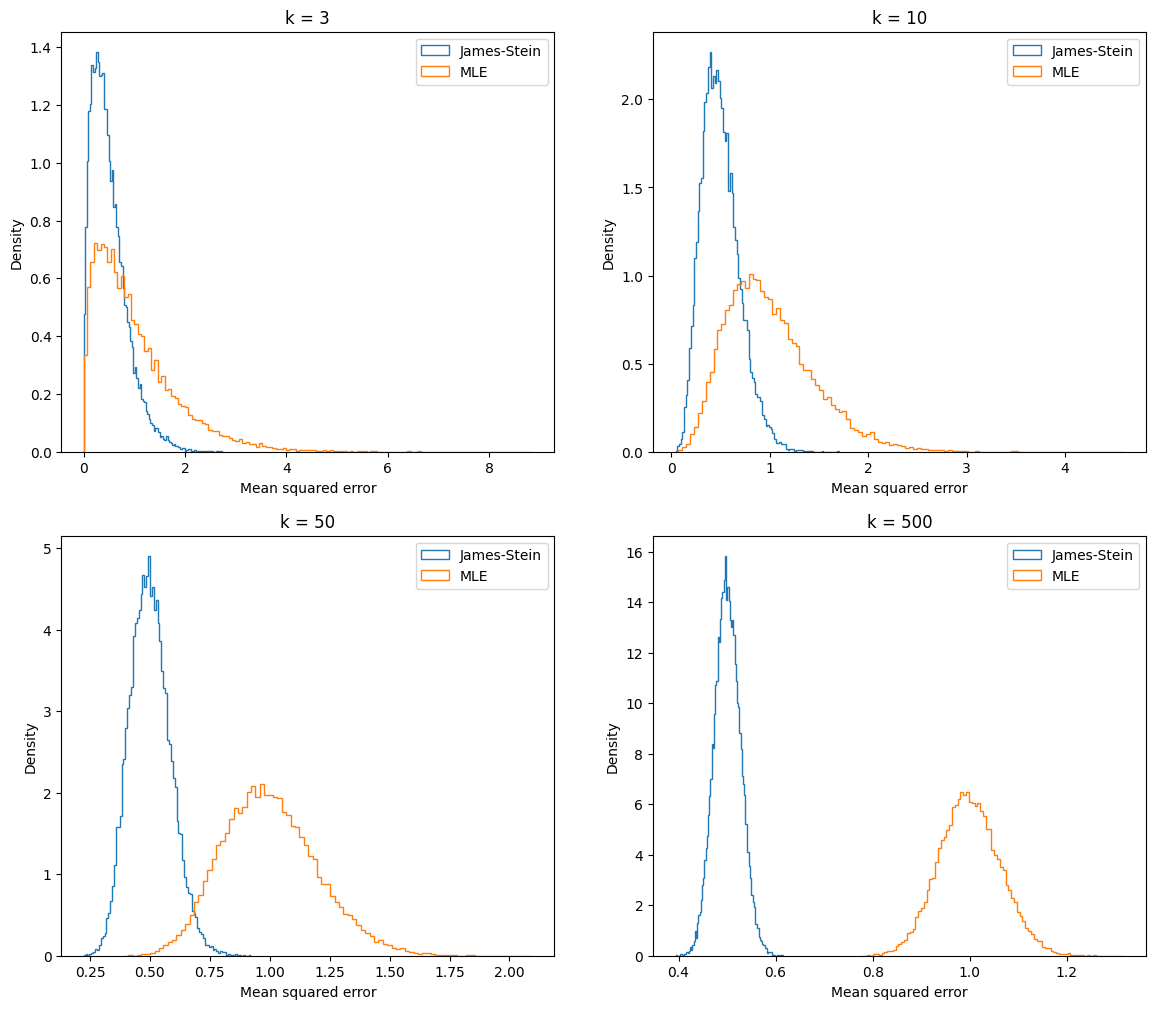
\includegraphics[scale=0.545]{../images/12-06a}
    \caption{Comparison of the mean squared error of the maximum likelihood
      estimator and the James-Stein estimator for different choices of $k$ under
      a true mean $\theta=(1,1,\ldots,1)$.}
  \end{figure}

  \begin{figure}[H]
    \centering
    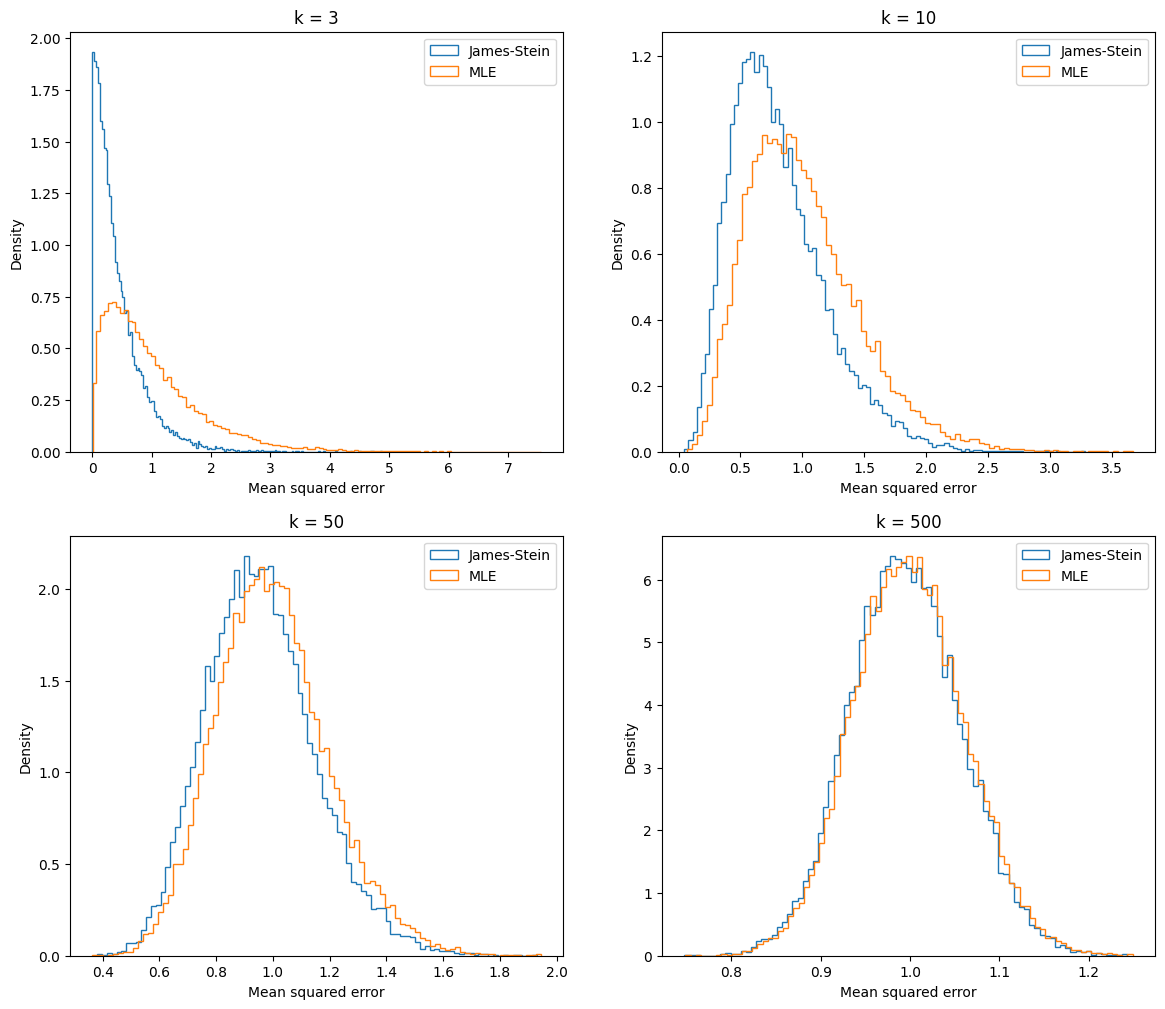
\includegraphics[scale=0.54]{../images/12-06b}
    \caption{Comparison of the mean squared error of the maximum likelihood
      and James-Stein estimators for different choices of $k$ under
      a true mean $\theta=(1,2,\ldots,k)$.}
  \end{figure}
\end{ex}